\subsection{UC8 - Inserimento \glossario{TICKET}}
\begin{itemize}
	\item \textbf{Identificativo}: UC8
	\item \textbf{Nome}: Inserimento \glossario{TICKET}
	\item\textbf{Descrizione Grafica}: 
	\begin{center}
		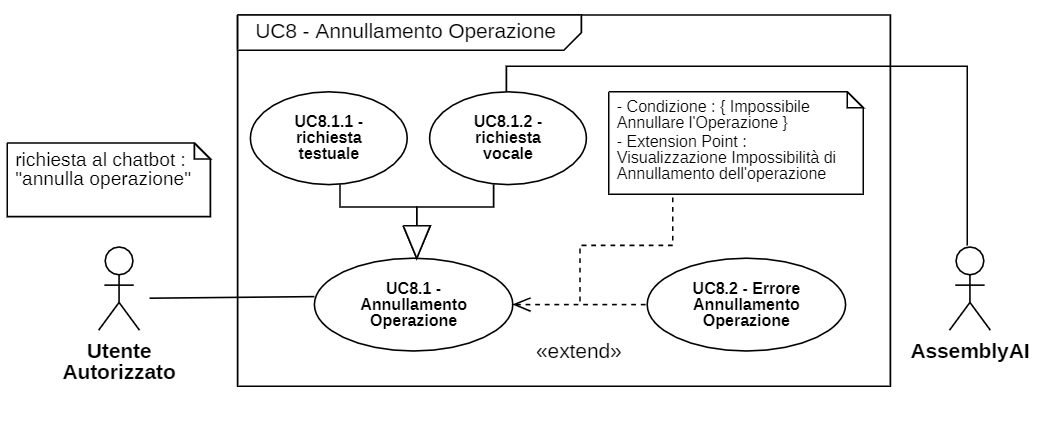
\includegraphics[scale=0.65]{images/UC8.png} 
	\end{center}

	\item \textbf{Attori}
	\begin{itemize} 
		\item \textit{Primari}: Utente autorizzato
		\item \textit{Secondari}: Nessuno 
	\end{itemize}
	\item \textbf{Descrizione}: L'utente vuole creare un nuovo \glossario{TICKET}. Dopo aver ricevuto la richiesta, il chatbot richiede le informazione necessarie al fine di creare un ticket. Il chatbot potrà dover chiedere ulteriori informazioni mancanti o, in caso di errore, comunicare all'utente l'impossibilità di creazione del \glossario{TICKET}.
	\item \textbf{Precondizione}: L'utente ha effettuato il login e si trova nella chat.
	\item \textbf{Postcondizione}: \glossario{TICKET} creato con successo.
	\item \textbf{Scenario principale}: \begin{enumerate}
		\item Utente inserisce un messaggio del tipo "Voglio creare un Nuovo Ticket";
		\item Chatbot chiede all'utente la descrizione;
		\item Chatbot chiede all'utente lo status;
		\item Chatbot chiede all'utente la priorità.		 
	\end{enumerate}
	\item \textbf{Estensioni}: \begin{itemize}
		\item Chatbot comunica che non è in grado di interpretare il comando;
		\item Chatbot comunica che l'azione non è andata a buon fine.
	\end{itemize}
\end{itemize}
\subsubsection{UC8.1 - Inserimento Oggetto per creazione \glossario{TICKET}}
\begin{itemize}
	\item \textbf{Identificativo}: UC8.1
	\item \textbf{Nome}: Inserimento Oggetto per creazione \glossario{TICKET} 
	\item \textbf{Attori}
	\begin{itemize} 
		\item \textit{Primari}: Utente autorizzato
		\item \textit{Secondari}: Nessuno
	\end{itemize}
	\item \textbf{Descrizione}: L'utente sta eseguendo il procedimento di creazione di un nuovo \glossario{TICKET}. Il chatbot richiede all'utente di inserire un Oggetto. 
	\item \textbf{Precondizione}: L'utente ha iniziato la procedura di creazione di un \glossario{TICKET}.
	\item \textbf{Postcondizione}: L'utente ha comunicato al chatbot l'oggetto del nuovo ticket.
	\item \textbf{Scenario principale}: \begin{enumerate}
		\item Chatbot interagisce con l'utente: "Indicare l'oggetto del ticket";
		\item Utente fornisce l'oggetto per la creazione del ticket.
	\end{enumerate}
	\item \textbf{Estensione}: Utente non ha inserito l'oggetto in maniera idonea per il chatbot.
		
\end{itemize}
\subsubsection{UC8.2 - Inserimento descrizione per creazione \glossario{TICKET}}
\begin{itemize}
	\item \textbf{Identificativo}: UC8.2
	\item \textbf{Nome}: Inserimento descrizione per creazione \glossario{TICKET} 
	\item \textbf{Attori}
	\begin{itemize} 
		\item \textit{Primari}: Utente autorizzato
		\item \textit{Secondari}: Nessuno
	\end{itemize}
	\item \textbf{Descrizione}:  Utente sta eseguendo il procedimento di creazione di un nuovo \glossario{TICKET}. Il chatbot richiede all'utente di inserire una descrizione. 
	\item \textbf{Precondizione}: Utente ha comunicato al chatbot l'oggetto del nuovo ticket.
	\item \textbf{Postcondizione}: Utente ha comunicato al chatbot la descrizione del nuovo ticket.
	\item \textbf{Scenario principale}: \begin{enumerate}
		\item Chatbot interagisce con l'utente: "Indicare la descrizione del ticket";
		\item Utente fornisce la descrizione per la creazione del ticket.
	\end{enumerate}
	\item \textbf{Estensione}: L'utente non ha inserito la descrizione in maniera idonea per il chatbot.
\end{itemize}
\subsubsection{UC8.3 - Inserimento Status per creazione \glossario{TICKET}}
\begin{itemize}
	\item \textbf{Identificativo}: UC8.3
	\item \textbf{Nome}: Inserimento Status per creazione \glossario{TICKET} 
	\item \textbf{Attori}
	\begin{itemize} 
		\item \textit{Primari}: Utente autorizzato
		\item \textit{Secondari}: Nessuno
	\end{itemize}
	\item \textbf{Descrizione}: L'utente sta eseguendo il procedimento di creazione di un nuovo \glossario{TICKET}. Il chatbot richiede all'utente di inserire uno status.
	\item \textbf{Precondizione}: l'utente ha comunicato al chatbot la descrizione del nuovo ticket.
	\item \textbf{Postcondizione}: l'utente ha comunicato al chatbot lo status del nuovo ticket.
	\item \textbf{Scenario principale}: \begin{enumerate}
		\item Chatbot interagisce con l'utente: "Indicare lo status del ticket";
		\item Utente fornisce lo status per la creazione del ticket.
	\end{enumerate}
	\item \textbf{Estensione}: L'utente non ha inserito lo status in maniera idonea per il chatbot. 
\end{itemize}
\subsubsection{UC8.4 - Inserimento priorità per creazione \glossario{TICKET}}
\begin{itemize}
	\item \textbf{Identificativo}: UC8.4
	\item \textbf{Nome}: Inserimento priorità per creazione \glossario{TICKET}
	\item \textbf{Attori}
	\begin{itemize} 
		\item \textit{Primari}: Utente autorizzato
		\item \textit{Secondari}: Nessuno
	\end{itemize}
	\item \textbf{Descrizione}: L'utente sta eseguendo il procedimento di creazione di un nuovo \glossario{TICKET}. Il chatbot richiede all'utente di assegnare una priorità.
	\item \textbf{Precondizione}: l'utente ha comunicato al chatbot lo status del nuovo ticket.
	\item \textbf{Postcondizione}: l'utente ha comunicato al chatbot la priorità del nuovo ticket.
	\item \textbf{Scenario principale}: \begin{enumerate}
		\item Chatbot interagisce con l'utente: "Assegnare una priorità al ticket";
		\item Utente assegna una priorità al ticket.
	\end{enumerate}
	\item \textbf{Estensione}: L'utente non ha inserito la priorità in maniera idonea per il chatbot.  
\end{itemize}
\subsubsection{UC8.5 - Visualizzazione errore inserimento oggetto}
\begin{itemize}
	\item \textbf{Identificativo}: UC8.5
	\item \textbf{Nome}: Visualizzazione errore inserimento oggetto 
	\item \textbf{Attori}
	\begin{itemize} 
		\item \textit{Primari}: Utente autorizzato
		\item \textit{Secondari}: Nessuno
	\end{itemize}
	\item \textbf{Descrizione}: È avvenuto un errore nell'inserimento dell'oggetto. Il chatbot mostra l'errore all'utente.
	\item \textbf{Precondizione}: L'utente sta eseguendo l'operazione di inserimento di un nuovo ticket. L'oggetto risulta essere inserito in un formato non valido. 
	\item \textbf{Postcondizione}: Chatbot mostra all'utente che l'oggetto non è stato inserito in maniera idonea per il chatbot.
	\item \textbf{Scenario principale}: \begin{enumerate}
		\item Chatbot mostra all'utente che è avvenuto un errore tramite chat: "Oggetto inserito in maniera non idonea".
		\end{enumerate}
\end{itemize}
\subsubsection{UC8.6 - Visualizzazione errore inserimento status}
\begin{itemize}
	\item \textbf{Identificativo}: UC8.6
	\item \textbf{Nome}: Visualizzazione errore inserimento status 
	\item \textbf{Attori}
	\begin{itemize} 
		\item \textit{Primari}: Utente autorizzato
		\item \textit{Secondari}: Nessuno
	\end{itemize}
	\item \textbf{Descrizione}: È avvenuto un errore nell'inserimento dello status. Il chatbot mostra l'errore all'utente.
	\item \textbf{Precondizione}: L'utente sta eseguendo l'operazione di inserimento di un nuovo ticket. Lo status risulta essere inserito in un formato non valido. 
	\item \textbf{Postcondizione}: Chatbot mostra all'utente che lo status non è stato inserito in maniera idonea per il chatbot.
	\item \textbf{Scenario principale}: 
	\begin{enumerate}
		\item Chatbot mostra all'utente che è avvenuto un errore tramite chat: "Status inserito in maniera non idonea". 
	\end{enumerate}
\end{itemize}
\subsubsection{UC8.7 - Visualizzazione errore inserimento priorità}
\begin{itemize}
	\item \textbf{Identificativo}: UC8.7
	\item \textbf{Nome}:  Visualizzazione errore inserimento priorità
	\item \textbf{Attori}
	\begin{itemize} 
		\item \textit{Primari}: Utente autorizzato
		\item \textit{Secondari}: Nessuno
	\end{itemize}
	\item \textbf{Descrizione}: È avvenuto un errore nell'inserimento della priorità. Il chatbot mostra l'errore all'utente.
	\item \textbf{Precondizione}: L'utente sta eseguendo l'operazione di inserimento di un nuovo ticket. La priorità risulta essere inserito in un formato non valido. 
	\item \textbf{Postcondizione}: Chatbot mostra all'utente che la priorità non è stata inserito in maniera idonea per il chatbot.
	\item \textbf{Scenario principale}: \begin{enumerate}
		\item Chatbot mostra all'utente che è avvenuto un errore tramite chat: "Priorità inserita in maniera non idonea".
	\end{enumerate}
\end{itemize}